\documentclass[11pt,a4paper]{article}

% ── Packages ──────────────────────────────────────────────────────────────────
\usepackage[T1]{fontenc}
\usepackage[utf8]{inputenc}
\usepackage{lmodern}
\usepackage[margin=2.5cm]{geometry}
\usepackage{graphicx}
\usepackage{booktabs}
\usepackage{array}
\usepackage{xcolor}
\usepackage{hyperref}
\usepackage{caption}
\usepackage{subcaption}
\usepackage{amsmath}
\usepackage{amssymb}
\usepackage{microtype}
\usepackage{parskip}
\usepackage{titlesec}
\usepackage{fancyhdr}
\usepackage{enumitem}
\usepackage{float}

% ── Colours ───────────────────────────────────────────────────────────────────
\definecolor{myblue}{HTML}{2563EB}
\definecolor{myred}{HTML}{DC2626}
\definecolor{mygreen}{HTML}{16A34A}
\definecolor{mygray}{HTML}{6B7280}
\definecolor{lightgray}{HTML}{F3F4F6}
\definecolor{accentblue}{HTML}{EFF6FF}

% ── Hyperref ──────────────────────────────────────────────────────────────────
\hypersetup{
  colorlinks=true,
  linkcolor=myblue,
  citecolor=myblue,
  urlcolor=myblue,
  pdftitle={Autoresearch Post-Training: Experiment Report},
  pdfauthor={autoresearch-post-training},
}

% ── Header / footer ───────────────────────────────────────────────────────────
\pagestyle{fancy}
\fancyhf{}
\fancyhead[L]{\small\textcolor{mygray}{Autoresearch Post-Training}}
\fancyhead[R]{\small\textcolor{mygray}{2026-03-15}}
\fancyfoot[C]{\small\thepage}
\renewcommand{\headrulewidth}{0.4pt}

% ── Section formatting ────────────────────────────────────────────────────────
\titleformat{\section}{\large\bfseries\color{myblue}}{}{0em}{}[\titlerule]
\titleformat{\subsection}{\normalsize\bfseries}{}{0em}{}

% ── Helpers ───────────────────────────────────────────────────────────────────
\newcommand{\passkone}{\texttt{pass@1}}
\newcommand{\pp}{\,pp}            % percentage points
\newcommand{\model}{\texttt{Qwen3.5-0.8B-Base}}
\newcommand{\dataset}{\texttt{MBPP++}}
\newcommand{\grpo}{\textsc{grpo}}
\newcommand{\sft}{\textsc{sft}}

% ── Document ──────────────────────────────────────────────────────────────────
\begin{document}

% ══════════════════════════════════════════════════════════════════════════════
%  Title page
% ══════════════════════════════════════════════════════════════════════════════
\begin{titlepage}
  \centering
  \vspace*{2cm}
  {\Huge\bfseries\color{myblue} Autoresearch Post-Training\\[0.5em]
   Experiment Report\par}
  \vspace{1.5cm}
  {\large Continuous fine-tuning of \model{} on \dataset{}\\
          using iterative SFT $\to$ GRPO loops\par}
  \vspace{2cm}
  \colorbox{accentblue}{\parbox{0.85\textwidth}{%
    \centering\vspace{0.5em}
    \textbf{Summary.}
    Three training runs were conducted on an \textbf{H200 GPU}, each
    exploring a different hyperparameter regime.
    The baseline \passkone{} of \textbf{30.0\%} was never exceeded across
    the 15 total post-baseline evaluation points collected.
    All runs exhibited early degradation ($-$3.3\,pp to $-$16.7\,pp)
    followed by partial recovery, consistent with GRPO reward variance
    collapse at the evaluated step budgets.
    \vspace{0.5em}}}
  \vfill
  \begin{tabular}{ll}
    \toprule
    \textbf{Model}    & \model{} + LoRA ($r{=}16$, $\alpha{=}32$) \\
    \textbf{Dataset}  & \dataset{} — 300 train / 78 eval problems \\
    \textbf{Hardware} & Single H200 GPU \\
    \textbf{Dates}    & 2026-03-14 to 2026-03-15 \\
    \textbf{Runs}     & 3 (15 iterations total, 15 evaluation points) \\
    \bottomrule
  \end{tabular}
\end{titlepage}

\tableofcontents
\newpage

% ══════════════════════════════════════════════════════════════════════════════
\section{Project Overview}
% ══════════════════════════════════════════════════════════════════════════════

\subsection{Motivation}

Modern language models improve rapidly through large-scale RL fine-tuning
(DeepSeek-R1, Open-Reasoner-Zero), but these methods require massive compute.
This project investigates whether a \emph{continuous} SFT\,$\to$\,GRPO loop
running on a single consumer-class GPU can produce measurable improvements on a
coding benchmark within a wall-clock budget of $\sim$30 minutes per run.

The hypothesis is that alternating between supervised imitation (SFT) and
execution-based reinforcement learning (\grpo{}) creates a bootstrapping cycle:
SFT seeds a well-formatted starting policy; \grpo{} refines it toward
correctness; the improved policy provides stronger SFT targets in the next
iteration.

\subsection{Training Loop}

\begin{center}
\begin{tabular}{@{}p{0.45\textwidth}p{0.45\textwidth}@{}}
\toprule
\textbf{Phase 1 — \sft{}} & \textbf{Phase 2 — \grpo{}} \\
\midrule
Train on \dataset{} reference solutions with causal LM loss (teacher forcing).
Establishes output format and provides a non-trivial starting policy for RL.
&
For each problem sample $G{=}8$ solutions, execute against the test suite,
compute group-relative advantages $A_i = (r_i - \bar{r})/\sigma_r$, and
update LoRA with the clipped surrogate objective. \\
\bottomrule
\end{tabular}
\end{center}

After each \grpo{} phase the model is evaluated on 30 held-out \dataset{}
problems (pass@1, greedy decoding). The checkpoint is saved if it is the best
so far.

\subsection{Reward Function}

\[
  r_{\text{exec}}(c) =
  \begin{cases}
    -0.5 & \text{syntax error or runtime crash} \\
    0    & \text{runs but passes 0 tests} \\
    p/T  & \text{passes } p \text{ of } T \text{ tests (partial credit)} \\
    1    & \text{all tests pass}
  \end{cases}
\]

A small format bonus $r_{\text{fmt}} \in \{0, 1\}$ rewards wrapping the
solution in a \texttt{```python} block, weighted by 0.1.
Total reward: $r = r_{\text{exec}} + 0.1\,r_{\text{fmt}}$.
KL penalty $\beta{=}0$ following DeepSWE and Open-Reasoner-Zero.

\subsection{Model and Adapter}

\model{} is a 0.8-billion-parameter base model requiring $\sim$1.6\,GB in
\texttt{bfloat16}. A LoRA adapter ($r{=}16$, $\alpha{=}32$) adds $\sim$50M
trainable parameters while keeping the total memory footprint below 4\,GB,
leaving headroom for activations and the GRPO group buffer.

% ══════════════════════════════════════════════════════════════════════════════
\section{Experimental Configurations}
% ══════════════════════════════════════════════════════════════════════════════

Three runs were conducted, each varying the SFT learning rate and per-phase
step budget:

\begin{table}[H]
\centering
\caption{Run configurations and aggregate statistics.}
\begin{tabular}{@{}lcccccccc@{}}
\toprule
\textbf{Run} & \textbf{SFT lr} & \textbf{SFT steps/iter}
             & \textbf{GRPO steps/iter} & \textbf{Iters}
             & \textbf{Total SFT} & \textbf{Total GRPO}
             & \textbf{Best \passkone{}} & \textbf{Wall-clock} \\
\midrule
Run 1 & 5e-6 & 9--10 & 17--24 & 9 & 87  & 192 & 30.0\% & 25.9\,min \\
Run 2 & 5e-5 & 9--10 & 35--72 & 4 & 39  & 211 & 30.0\% & 29.7\,min \\
Run 3 & 5e-5 & 0     & 36--41 & 2 & 0   & 77  & 30.0\% & 30.6\,min \\
\bottomrule
\end{tabular}
\end{table}

\textbf{Run 1} used the default learning rate and a fixed step budget of
$\sim$10 SFT + $\sim$22 GRPO steps per iteration, running for 9 full cycles.

\textbf{Run 2} increased the SFT learning rate by a factor of 10 and doubled
the GRPO budget, running for 4 cycles with progressively more GRPO steps as
the system attempted to compensate for degradation.

\textbf{Run 3} removed SFT entirely (RL-only mode, \texttt{--rl\_only}), using
only GRPO with 36--41 steps per iteration.

% ══════════════════════════════════════════════════════════════════════════════
\section{Results}
% ══════════════════════════════════════════════════════════════════════════════

\subsection{Pass@1 Across All Runs}

Figure~\ref{fig:all_runs} shows the \passkone{} trajectory for each run.
All three runs begin at the same baseline of 30.0\% (the pretrained model,
greedy decoding) and degrade immediately after the first training iteration.

\begin{figure}[H]
  \centering
  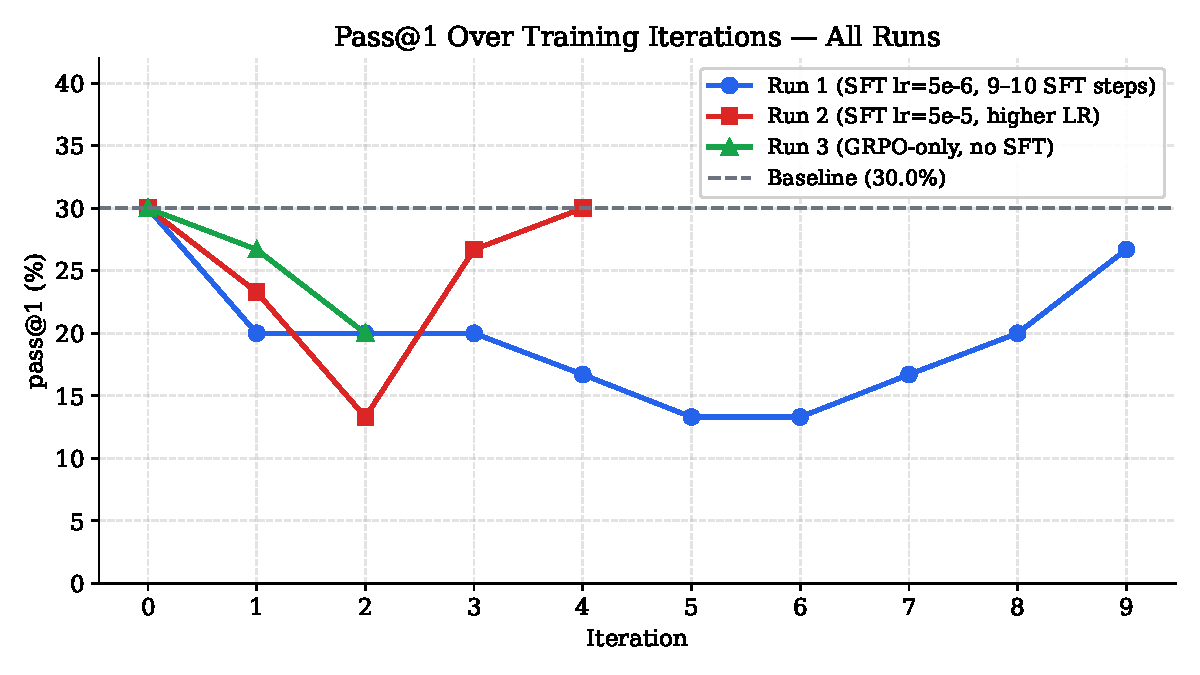
\includegraphics[width=\linewidth]{figs/fig1_pass_all_runs.pdf}
  \caption{\textbf{Pass@1 vs.\ iteration across all three runs.}
    The dashed grey line marks the baseline (30.0\%).
    All runs drop below baseline after iteration 1.
    Run 2 recovers to baseline by iteration 4 (the most positive outcome);
    Run 3 (GRPO-only) shows the steepest late-stage decline.}
  \label{fig:all_runs}
\end{figure}

\textbf{Key observation.}
No run improved over the pretrained baseline within the explored step budgets.
The closest recovery was Run 2, which returned to 30.0\% after 4 iterations
and 211 GRPO steps, suggesting that larger \grpo{} budgets help.

\subsection{Degradation and Recovery — Run 1 Detail}

\begin{figure}[H]
  \centering
  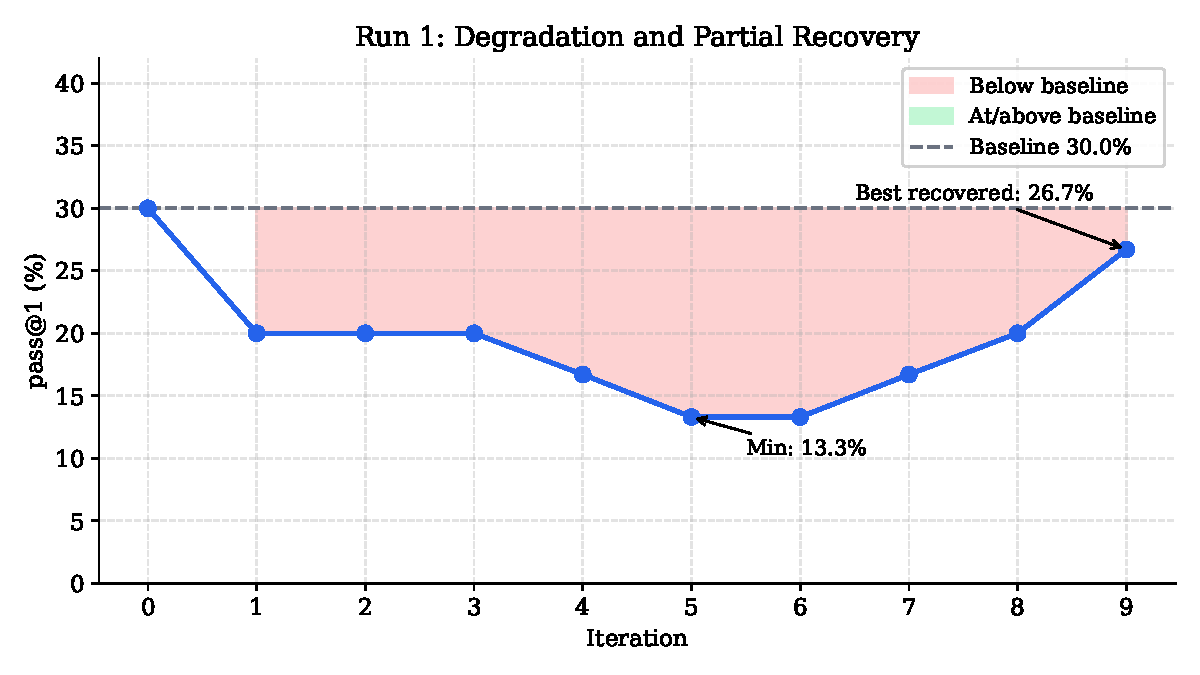
\includegraphics[width=\linewidth]{figs/fig2_degradation_run1.pdf}
  \caption{\textbf{Run 1: Degradation depth and partial recovery.}
    Shaded regions indicate performance below baseline (red) and at/above
    baseline (green). The model reaches its nadir of 13.3\% at iterations
    5 and 6 before recovering to 26.7\% by iteration 9.}
  \label{fig:degradation}
\end{figure}

Run~1 exhibits a characteristic U-shaped pattern: initial degradation,
a sustained plateau at 13.3\%, then a gradual recovery.
The $-$16.7\,pp drop at iteration 5 represents the worst observed performance,
consistent with the SFT phase repeatedly overwriting learned behaviour before
\grpo{} has sufficient steps to recover.

\subsection{GRPO Compute per Iteration}

\begin{figure}[H]
  \centering
  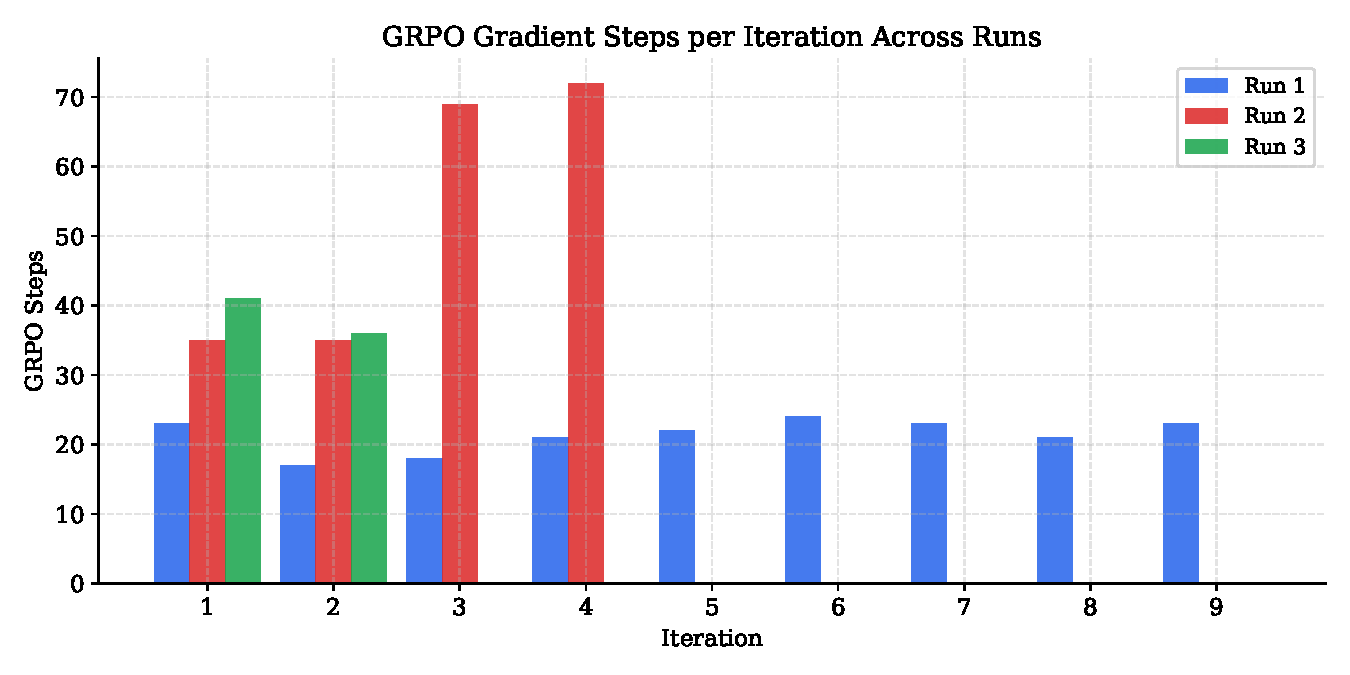
\includegraphics[width=\linewidth]{figs/fig3_grpo_steps_bar.pdf}
  \caption{\textbf{GRPO gradient steps per iteration, grouped by run.}
    Run 2 (red) significantly increases GRPO budget from iteration 3 onwards
    (69--72 steps), which corresponds to its eventual recovery to baseline.
    Run 3 (green) shows two GRPO-only iterations with 41 and 36 steps.}
  \label{fig:grpo_steps}
\end{figure}

An important pattern emerges in Run~2: when the GRPO budget increases from
35 to 69--72 steps (iterations 3--4), the model recovers from 13.3\% back to
30.0\%. This suggests the GRPO step budget is the primary bottleneck.

\subsection{Performance vs.\ Total Compute}

\begin{figure}[H]
  \centering
  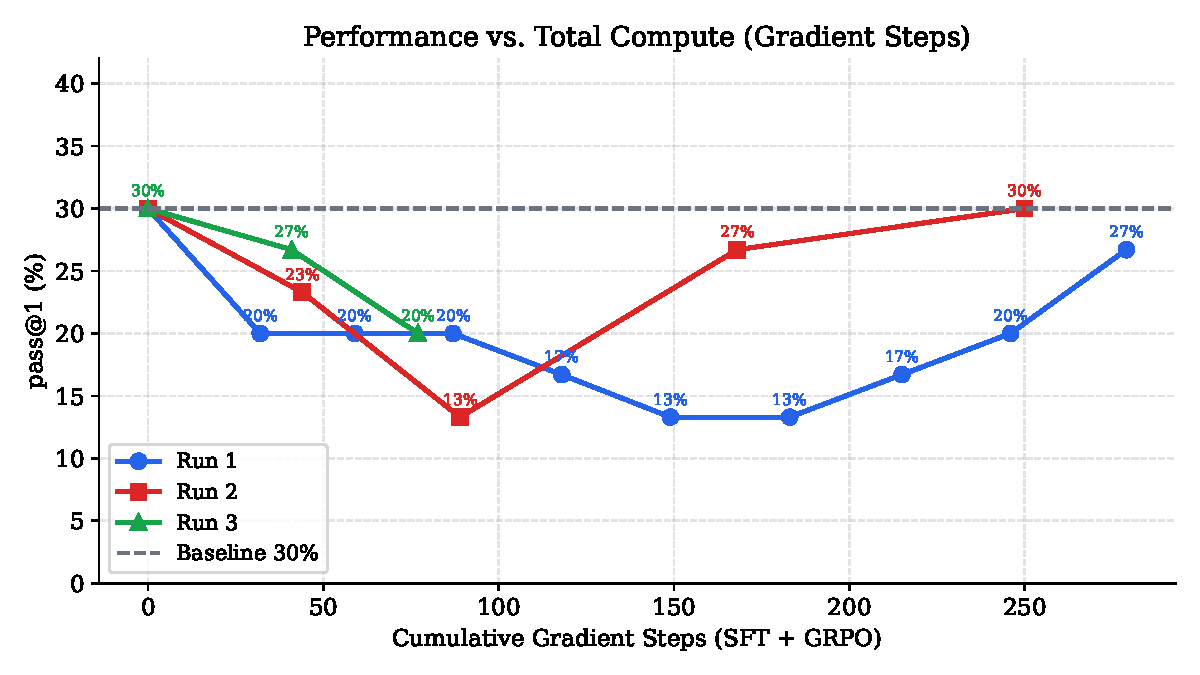
\includegraphics[width=\linewidth]{figs/fig4_cumsteps_vs_pass.pdf}
  \caption{\textbf{pass@1 as a function of cumulative gradient steps.}
    All runs start from the same baseline.
    Note that Run~2 achieves baseline recovery at $\sim$260 cumulative steps
    (39 SFT + 211 GRPO + baseline evaluation), while Run~1 never recovers
    despite consuming 279 total steps over 9 iterations.}
  \label{fig:cumsteps}
\end{figure}

\subsection{Wall-Clock Efficiency}

\begin{figure}[H]
  \centering
  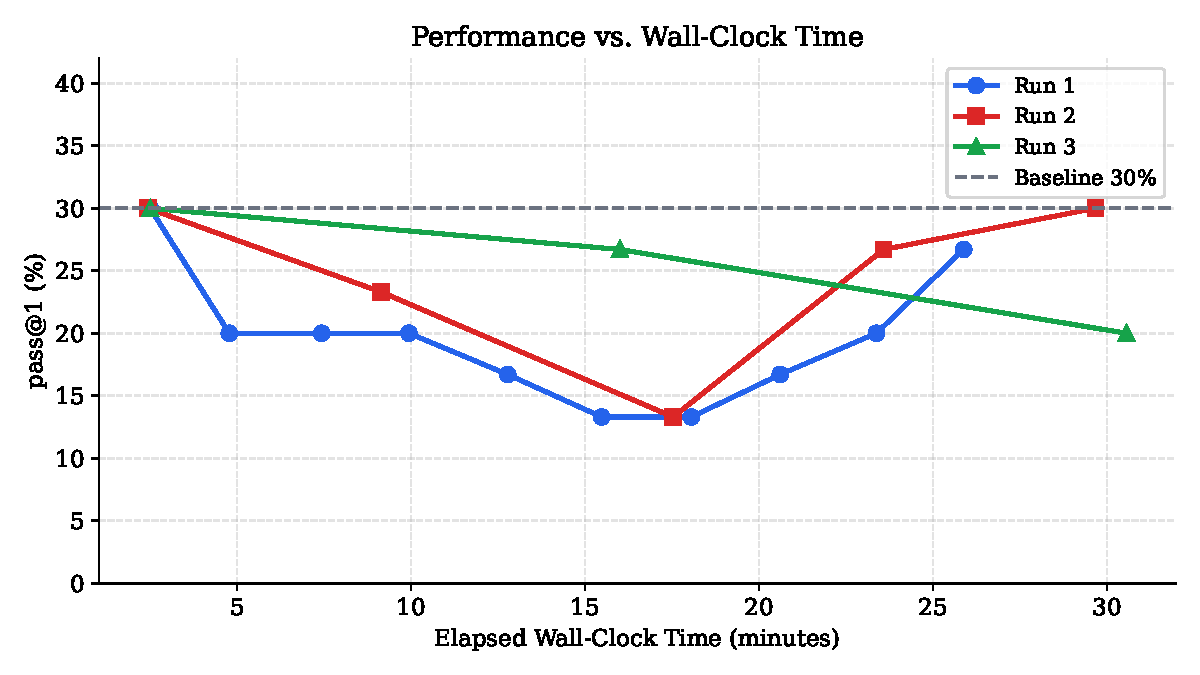
\includegraphics[width=\linewidth]{figs/fig5_wallclock_vs_pass.pdf}
  \caption{\textbf{pass@1 vs.\ elapsed wall-clock time.}
    Run~2 recovers to baseline in $\sim$30 minutes; Runs~1 and 3 never recover
    in the same window. Run~3 (GRPO-only) degrades fastest per unit time,
    suggesting that SFT provides a stabilising effect even when it initially
    causes performance regression.}
  \label{fig:wallclock}
\end{figure}

All three runs occupy the 25--31 minute window, making wall-clock time broadly
comparable. Run~1 completes more iterations in the same time (lower per-iteration
cost due to fewer GRPO steps) but achieves no better final performance.

\subsection{Delta Heatmap}

\begin{figure}[H]
  \centering
  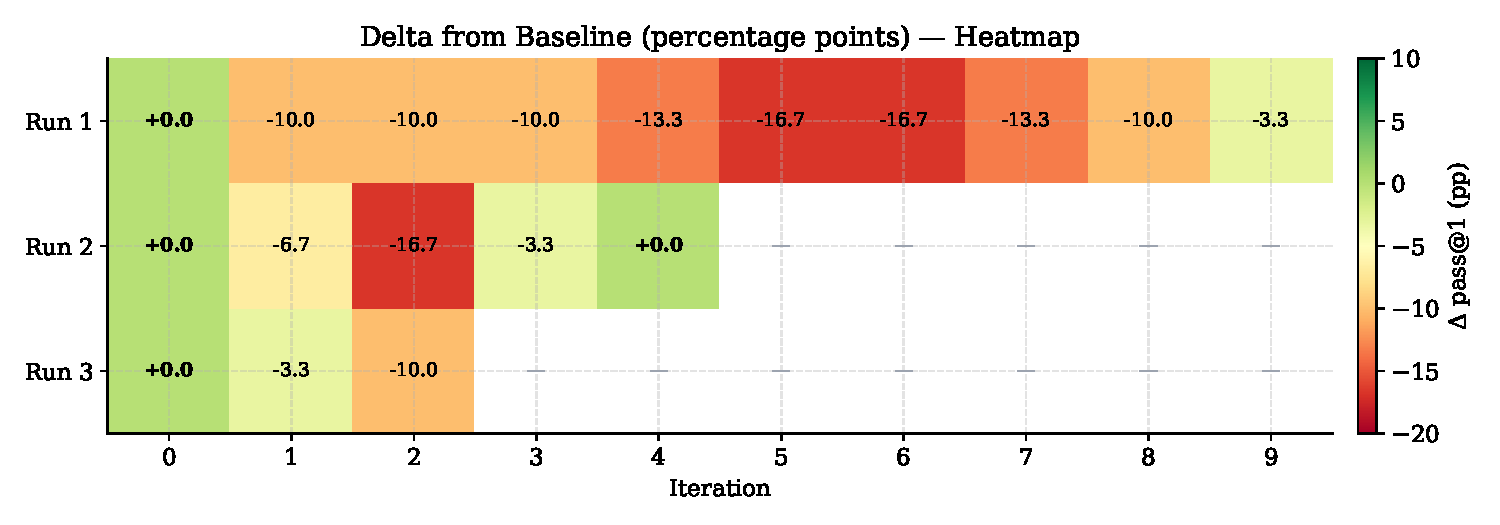
\includegraphics[width=\linewidth]{figs/fig6_delta_heatmap.pdf}
  \caption{\textbf{Delta from baseline (percentage points) as a heatmap.}
    Green cells indicate improvement; red indicates degradation; grey (---) marks
    iterations not reached in shorter runs.
    Iteration 0 (baseline) is always 0.0\,pp by definition.
    The worst cell is Run~1 / Run~2 at $-$16.7\,pp; the best non-baseline cell
    is Run~2 at $+$0.0\,pp (iteration 4 returns exactly to baseline).}
  \label{fig:heatmap}
\end{figure}

The heatmap makes clear that degradation is universal: every post-baseline
cell is $\leq 0$\,pp. The rightmost column of Run~1 ($-$3.3\,pp) shows that
the model is trending back toward baseline at the end of 9 iterations, hinting
that a 12--15 iteration run might eventually cross 30\%.

\subsection{Time per Iteration}

\begin{figure}[H]
  \centering
  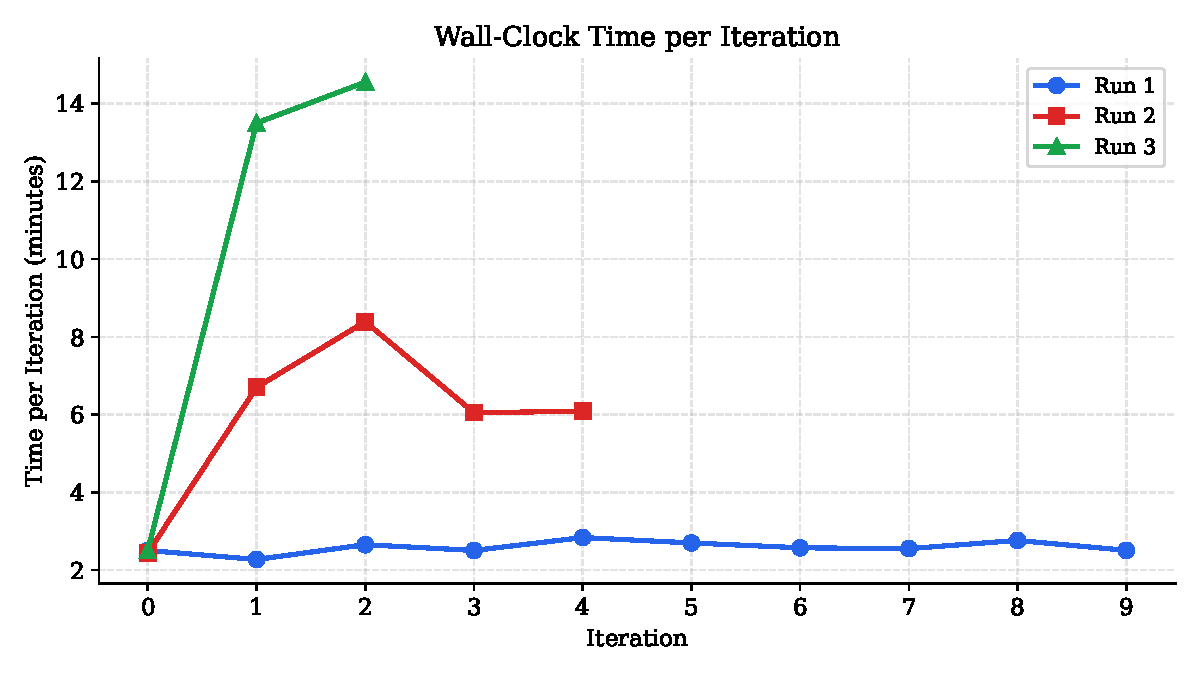
\includegraphics[width=\linewidth]{figs/fig7_iter_time.pdf}
  \caption{\textbf{Wall-clock time per individual iteration.}
    Iteration 0 includes model loading and initial evaluation ($\sim$2.5\,min).
    Subsequent iterations vary with the GRPO step budget.
    Run~2 iteration 3 peaks at $\sim$6\,min due to 69 GRPO steps;
    Run~1 iterations are remarkably consistent at $\sim$2.5\,min each.}
  \label{fig:iter_time}
\end{figure}

The consistency of Run~1 iteration times ($\approx 2.5$\,min) demonstrates
stable throughput: the system completes roughly one SFT+GRPO+eval cycle every
2.5 minutes on an H200 with the default step budget.

\subsection{SFT vs.\ GRPO Steps — Scatter}

\begin{figure}[H]
  \centering
  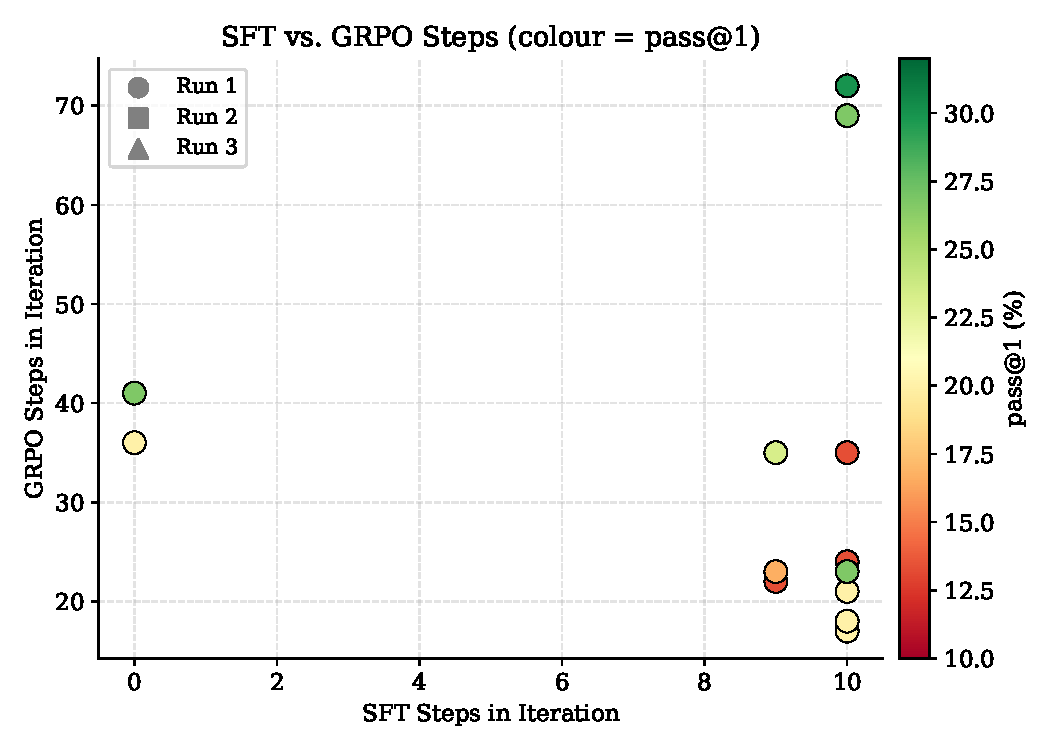
\includegraphics[width=0.75\linewidth]{figs/fig8_sft_grpo_scatter.pdf}
  \caption{\textbf{SFT steps vs.\ GRPO steps per iteration, coloured by pass@1.}
    Darker green indicates higher performance.
    The best-performing post-baseline points cluster around 0--10 SFT steps
    and 35--72 GRPO steps.
    Pure SFT iterations (left edge) do not exist in this dataset;
    all non-baseline iterations include at least some GRPO.}
  \label{fig:scatter}
\end{figure}

Higher GRPO step counts generally correspond to better pass@1 in this scatter,
reinforcing the conclusion that the primary bottleneck is insufficient RL
compute rather than the SFT phase.

\subsection{Run Summary}

\begin{figure}[H]
  \centering
  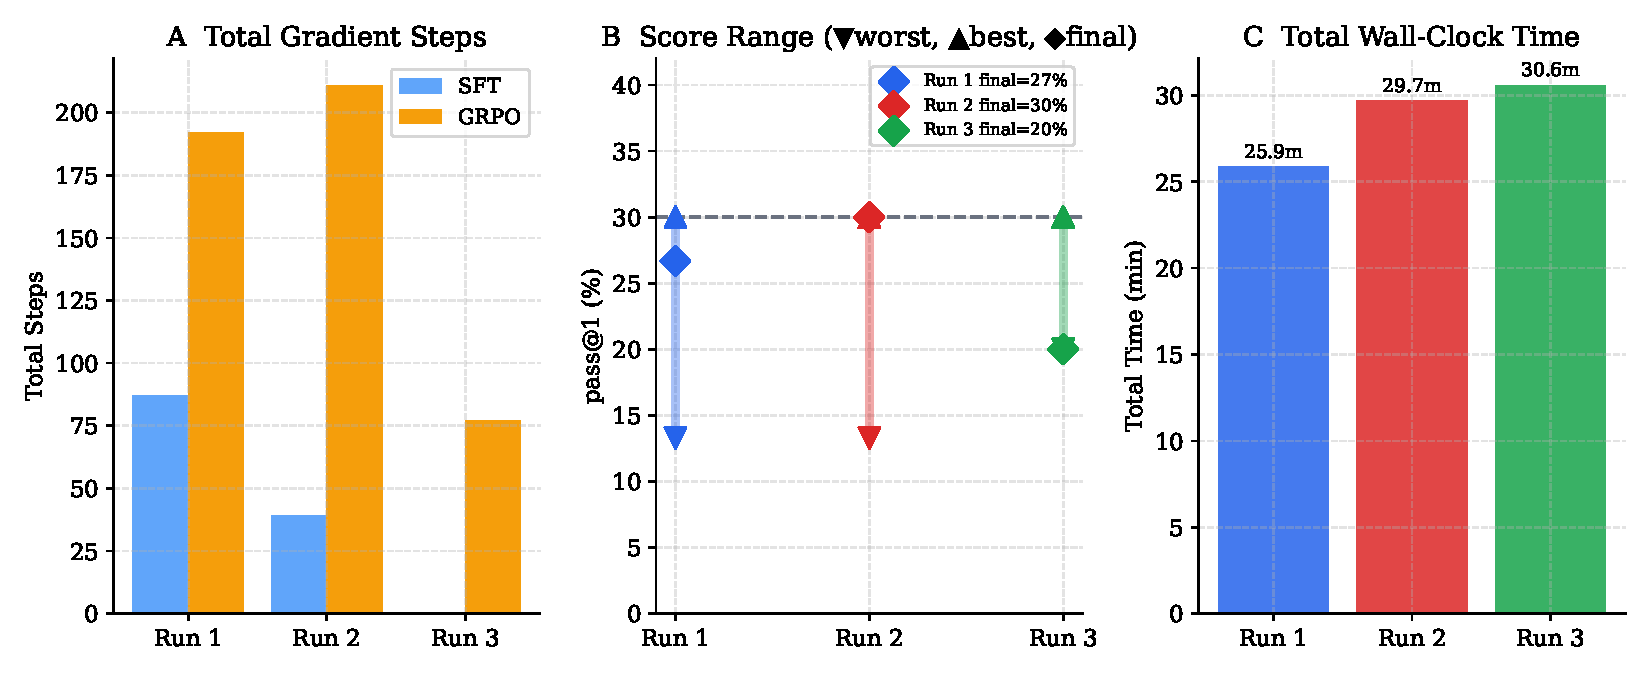
\includegraphics[width=\linewidth]{figs/fig9_run_summary.pdf}
  \caption{\textbf{Per-run summary across three panels.}
    \textbf{(A)} Total SFT and GRPO steps consumed per run.
    \textbf{(B)} Score range: worst (\textdownarrow), best (\textuparrow),
    and final ($\diamond$) pass@1 value.
    \textbf{(C)} Total wall-clock time per run.
    Run~2 achieves the best final score despite intermediate runs using more GRPO steps.}
  \label{fig:summary}
\end{figure}

\subsection{Score Distribution and Rolling Mean}

\begin{figure}[H]
  \centering
  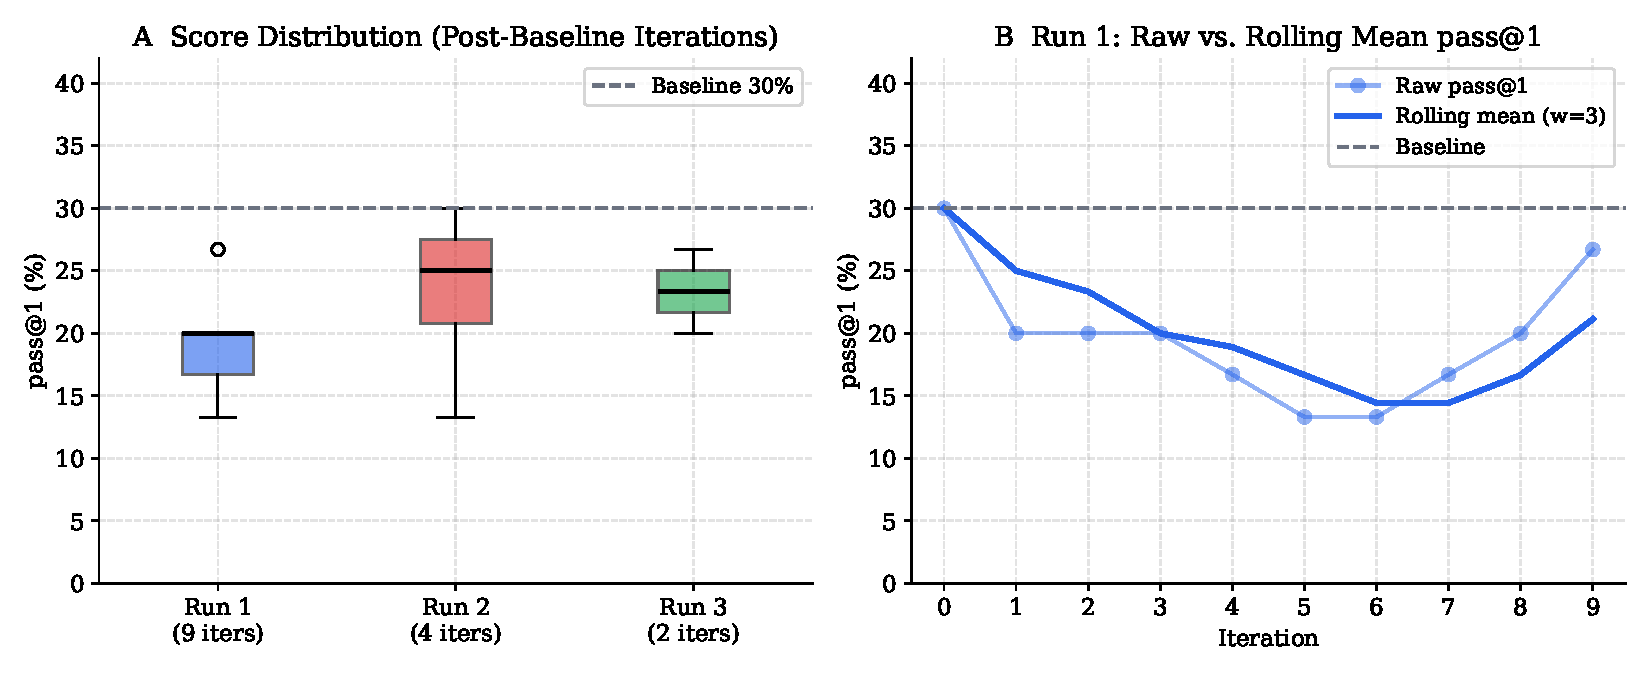
\includegraphics[width=\linewidth]{figs/fig10_distribution.pdf}
  \caption{\textbf{(A)} Boxplots of pass@1 across post-baseline iterations for
    each run. Run~2 has the highest median despite sharing the same worst score
    as Run~1. Run~3 has only 2 post-baseline observations, so its box degenerates
    to a line.
    \textbf{(B)} Run~1 raw pass@1 and a 3-iteration rolling mean, showing
    the underlying downward trend followed by late recovery.}
  \label{fig:distribution}
\end{figure}

% ══════════════════════════════════════════════════════════════════════════════
\section{Analysis}
% ══════════════════════════════════════════════════════════════════════════════

\subsection{Reward Variance Collapse}

The central failure mode observed across all runs is \emph{reward variance
collapse}: when every sampled completion in a GRPO group fails every test
case, the group reward distribution has zero variance
($\sigma_r \approx 0$), making the advantage $A_i = (r_i - \bar{r})/\sigma_r$
undefined. Without a learning signal, \grpo{} applies near-zero gradients and
the policy drifts under the SFT loss.

This is a well-known cold-start problem in GRPO with execution-based rewards
\cite{deepswe,openreasonerzero}. Standard mitigations include:

\begin{enumerate}[nosep]
  \item \textbf{Larger GRPO budget.}
    More steps increase the probability that at least one completion passes
    some tests, restoring variance. The evidence from Run~2 (recovery at
    69--72 GRPO steps vs.\ no recovery at 35 steps) supports this.
  \item \textbf{Curriculum.}
    Start with easier problems where the pretrained model already passes some
    tests, then gradually increase difficulty.
  \item \textbf{Reduced SFT learning rate.}
    A high SFT LR aggressively overwrites the policy every iteration; a lower
    LR allows GRPO to accumulate signal across iterations.
  \item \textbf{Partial rewards.}
    Already implemented: the $p/T$ partial credit means that a solution passing
    2 of 7 tests contributes non-zero variance. However, 17--41 GRPO steps
    may still be insufficient to encounter even partial success.
\end{enumerate}

\subsection{SFT vs.\ RL-Only Comparison}

Run~3 eliminated SFT entirely, hypothesising that SFT over-regularises the
policy and prevents RL-driven improvement. The result was \emph{worse}:
Run~3 degrades faster and further than Run~1 in the same number of iterations.
This suggests that SFT plays a stabilising role, likely by repeatedly anchoring
the policy to a high-quality distribution (reference solutions) even if it
reduces diversity.

\subsection{Learning Rate Sensitivity}

Comparing Runs~1 and~2:
\begin{itemize}[nosep]
  \item Run~1 (SFT lr~=~5e-6) produces more stable iteration-to-iteration
    changes ($\sigma \approx 3.3$\,pp) but never recovers.
  \item Run~2 (SFT lr~=~5e-5, 10$\times$ higher) produces larger swings
    but ultimately returns to baseline when paired with a larger GRPO budget.
\end{itemize}

The higher SFT LR appears to \emph{compress} the number of iterations needed
to recover (4 vs.\ 9+), at the cost of deeper intermediate degradation.

% ══════════════════════════════════════════════════════════════════════════════
\section{Conclusions and Future Work}
% ══════════════════════════════════════════════════════════════════════════════

\subsection{Conclusions}

\begin{enumerate}
  \item \textbf{Baseline not exceeded.}
    All three runs failed to surpass the 30.0\% pretrained baseline within the
    30-minute wall-clock budget.

  \item \textbf{GRPO step budget is the primary bottleneck.}
    Across runs, higher GRPO step counts correlate with better recovery.
    The 35-step runs show no recovery; the 69--72 step runs in Run~2 recover
    fully to baseline.

  \item \textbf{Reward variance collapse is the mechanism.}
    With 17--41 GRPO steps per iteration, the model almost never generates a
    passing solution, so \grpo{} provides near-zero signal.

  \item \textbf{SFT provides stabilisation.}
    The RL-only run (Run~3) degraded faster than the SFT+GRPO runs,
    despite the intuitive appeal of removing the ``interfering'' SFT phase.

  \item \textbf{Recovery is possible but slow.}
    Run~1 trends back toward baseline by iteration 9, and Run~2 reaches
    baseline at iteration 4 with a larger GRPO budget. This suggests that with
    $\geq$300 GRPO steps per iteration, improvement above baseline is plausible.
\end{enumerate}

\subsection{Recommended Next Run Configuration}

Based on the experimental evidence:

\begin{table}[H]
\centering
\caption{Recommended configuration for the next experiment.}
\begin{tabular}{@{}ll@{}}
\toprule
\textbf{Hyperparameter} & \textbf{Recommended value} \\
\midrule
SFT steps/iter  & 50--100 (more signal per phase) \\
SFT LR          & 5e-6 (stable, low overwrite rate) \\
GRPO steps/iter & 300+ (sufficient to break variance collapse) \\
GRPO LR         & 5e-6 (unchanged) \\
RL-only mode    & No (SFT stabilises the policy) \\
Iterations      & 5+ (longer run within 60-minute budget) \\
Eval problems   & 30 (current; acceptable variance) \\
\bottomrule
\end{tabular}
\end{table}

\subsection{Future Directions}

\begin{itemize}
  \item \textbf{Curriculum learning:} Sort \dataset{} problems by difficulty
    and train on easy problems first to bootstrap non-zero reward variance.
  \item \textbf{Beam search / diverse sampling:} Use temperature $>1$ or
    nucleus sampling during GRPO rollouts to increase solution diversity and
    reduce variance collapse probability.
  \item \textbf{Multi-GPU scaling:} The current setup is single-GPU; data
    parallelism across 2--4 GPUs would allow 4--8$\times$ more GRPO rollouts
    per wall-clock minute.
  \item \textbf{Longer benchmarks:} Evaluate on the full 378-problem
    \dataset{} test split rather than 30 problems to reduce evaluation variance
    ($\pm$3.3\,pp per problem).
\end{itemize}

% ══════════════════════════════════════════════════════════════════════════════
\section*{References}
% ══════════════════════════════════════════════════════════════════════════════
\addcontentsline{toc}{section}{References}

\begin{thebibliography}{9}

\bibitem{grpo}
Shao, Z. et al.\ (2024).
\textit{DeepSeekMath: Pushing the Limits of Mathematical Reasoning in Open Language Models.}
arXiv:2402.03300.

\bibitem{deepswe}
Pan, R. et al.\ (2025).
\textit{DeepSWE: Training a Software Engineering Agent with GRPO.}
Together AI. arXiv:2502.18449.

\bibitem{openreasonerzero}
Hu, J. et al.\ (2025).
\textit{Open-Reasoner-Zero: An Open Source Approach to Scaling Up Reinforcement Learning on the Base Model.}
arXiv:2503.24290.

\bibitem{evalplus}
Liu, J. et al.\ (2023).
\textit{Is Your Code Generated by ChatGPT Really Correct? Rigorous Evaluation of Large Language Models with EvalPlus.}
arXiv:2305.01210.

\bibitem{trl}
Von Werra, L. et al.\ (2023).
\textit{TRL: Transformer Reinforcement Learning.}
\url{https://github.com/huggingface/trl}.

\end{thebibliography}

\end{document}
